\documentclass[journal,12pt,twocolumn]{IEEEtran}
\usepackage{amsthm}
\usepackage{gensymb}
\usepackage{setspace}
\singlespacing
\usepackage[cmex10]{amsmath}
\usepackage{bm}

\usepackage{cases}
\usepackage{mathrsfs}
\usepackage{cite}
\usepackage{stfloats}
\usepackage{mathtools}
\usepackage[breaklinks=true]{hyperref}
\usepackage{graphicx}
\usepackage{subfig}
\usepackage{txfonts}
\usepackage{longtable}
\usepackage{multirow}
\usepackage{tfrupee}
\newcommand*{\Comb}[2]{{}^{#1}C_{#2}}%
\usepackage{enumitem}
\usepackage{tikz}
\usepackage{steinmetz}
\usepackage{verbatim}
\usepackage{circuitikz}
\usepackage{tkz-euclide}





\usetikzlibrary{calc,math}
\usepackage{listings}
    \usepackage{color}                                            %%
    \usepackage{array}                                            %%
    \usepackage{longtable}                                        %%
    \usepackage{calc}                                             %%
    \usepackage{multirow}                                         %%
    \usepackage{hhline}                                           %%
    \usepackage{ifthen}                                           %%
    \usepackage{lscape}     
\usepackage{multicol}
\usepackage{chngcntr}

\DeclareMathOperator*{\Res}{Res}

\renewcommand\thesection{\arabic{section}}
\renewcommand\thesubsection{\thesection.\arabic{subsection}}
\renewcommand\thesubsubsection{\thesubsection.\arabic{subsubsection}}

\renewcommand \thesectiondis{\arabic{section}}
\renewcommand\thesubsectiondis{\thesectiondis.\arabic{subsection}}
\renewcommand\thesubsubsectiondis{\thesubsectiondis.\arabic{subsubsection}}


\hyphenation{op-tical net-works semi-conduc-tor}
\def\inputGnumericTable{}                                 %%
\providecommand{\nCr}[2]{\,^{#1}C_{#2}}
\providecommand{\nPr}[2]{\,^{#1}P_{#2}}
\lstset{
%language=C,
frame=single, 
breaklines=true,
columns=fullflexible
}
\begin{document}

\newcommand{\BEQA}{\begin{eqnarray}}
\newcommand{\EEQA}{\end{eqnarray}}
\newcommand{\define}{\stackrel{\triangle}{=}}
\bibliographystyle{IEEEtran}
\raggedbottom
\setlength{\parindent}{0pt}
\providecommand{\mbf}{\mathbf}
\providecommand{\pr}[1]{\ensuremath{\Pr\left(#1\right)}}
\providecommand{\qfunc}[1]{\ensuremath{Q\left(#1\right)}}
\providecommand{\sbrak}[1]{\ensuremath{{}\left[#1\right]}}
\providecommand{\lsbrak}[1]{\ensuremath{{}\left[#1\right.}}
\providecommand{\rsbrak}[1]{\ensuremath{{}\left.#1\right]}}
\providecommand{\brak}[1]{\ensuremath{\left(#1\right)}}
\providecommand{\lbrak}[1]{\ensuremath{\left(#1\right.}}
\providecommand{\rbrak}[1]{\ensuremath{\left.#1\right)}}
\providecommand{\cbrak}[1]{\ensuremath{\left\{#1\right\}}}
\providecommand{\lcbrak}[1]{\ensuremath{\left\{#1\right.}}
\providecommand{\rcbrak}[1]{\ensuremath{\left.#1\right\}}}

\theoremstyle{remark}
\newtheorem{rem}{Remark}
\newcommand{\sgn}{\mathop{\mathrm{sgn}}}
\providecommand{\abs}[1]{\vert#1\vert}
\providecommand{\res}[1]{\Res\displaylimits_{#1}} 
\providecommand{\norm}[1]{\lVert#1\rVert}
%\providecommand{\norm}[1]{\lVert#1\rVert}
\providecommand{\mtx}[1]{\mathbf{#1}}
\providecommand{\mean}[1]{E[ #1 ]}
\providecommand{\fourier}{\overset{\mathcal{F}}{ \rightleftharpoons}}
%\providecommand{\hilbert}{\overset{\mathcal{H}}{ \rightleftharpoons}}
\providecommand{\system}{\overset{\mathcal{H}}{ \longleftrightarrow}}
	%\newcommand{\solution}[2]{\textbf{Solution:}{#1}}
\newcommand{\solution}{\noindent \textbf{Solution: }}
\newcommand{\cosec}{\,\text{cosec}\,}
\providecommand{\dec}[2]{\ensuremath{\overset{#1}{\underset{#2}{\gtrless}}}}
\newcommand{\myvec}[1]{\ensuremath{\begin{pmatrix}#1\end{pmatrix}}}
\newcommand{\mydet}[1]{\ensuremath{\begin{vmatrix}#1\end{vmatrix}}}
\numberwithin{equation}{subsection}
\makeatletter
\@addtoreset{figure}{problem}
\makeatother
\let\StandardTheFigure\thefigure
\let\vec\mathbf
\renewcommand{\thefigure}{\theproblem}
\def\putbox#1#2#3{\makebox[0in][l]{\makebox[#1][l]{}\raisebox{\baselineskip}[0in][0in]{\raisebox{#2}[0in][0in]{#3}}}}
     \def\rightbox#1{\makebox[0in][r]{#1}}
     \def\centbox#1{\makebox[0in]{#1}}
     \def\topbox#1{\raisebox{-\baselineskip}[0in][0in]{#1}}
     \def\midbox#1{\raisebox{-0.5\baselineskip}[0in][0in]{#1}}
\vspace{3cm}
\title{Assignment1}%number
\author{CS20Btech11035 -NYALAPOGULA MANASWINI}
\maketitle
\newpage
\bigskip

\renewcommand{\thefigure}{\theenumi}
\renewcommand{\thetable}{\theenumi}

Download python code from 
\begin{lstlisting}
https://github.com/N-Manaswini23/assignment1/blob/main/assignment1%20(2).py
\end{lstlisting}
%



\section*{ QUESTION 3.3:}
Suppose X has a binomial
 distribution . Show that $X = 3$ is the most likely outcome.(Hint : $P(X = 3)$ is the maximum among all $P(x_i$), ($x_i$= 0,1,2,3,4,5,6).Assume $p=\frac{1}{2}$ 
 \\
\section*{SOLUTION}:\\
Let X be a binomial random variable which has probability  $p=\frac{1}{2}$ 
 \begin{align}
p(X)=\frac{1}{2} \label{1}
 \end{align}
Given number of times event(X) is\\
 performed$(n)=6$
 \begin{align}
 n(x)=6 \label{2}
 \end{align}
Given probability of event$(p)= \frac{1}{2}$\\
Probability that event(X) does not \\occur is
$(1-p)=1-\frac{1}{2}=\frac{1}{2} $
 \begin{align}
1-p(x)=\frac{1}{2}\label{3}
 \end{align}
We know that binomial probability
\begin{align}
\pr{X=k} = \Comb{n}{k} p^k({1-p})^{n-k}  \label{4} 
\end{align}
For $\pr{X=k}$ to be most likely outcome(highest probability),
 $\pr{X=k}$  should be maximum ,where\\
$ k=\{0,1,2,3,4,5,6\}$\\
To find maximum of  $\pr{X=k}$  ,let us  apply \\logarithm on both sides for equation \eqref{4} and then diffenrentiate it with respect
to $p$.
\begin{align}
\log  \pr{X=k} &=\log  \Comb{n}{k} \times p^k\times ({1-p})^{n-k} \\
&=\log \Comb{n}{k} +k \times \log p \notag \\
 &+(n-k)\times log (1-p) \label{5}
\end{align}
Differentaiate eq \eqref{5} with respect to p

\begin{align}
\frac{\mathrm{d} \log \pr{X=k} }{\mathrm{d} p}&=\frac{\mathrm{d} \log  \Comb{n}{k} }{\mathrm{d}p}+k\times  \frac{\mathrm{d}\log p}{\mathrm{d} p} \\
     &+(n-k) \times \frac{\mathrm{d}\log (1-p)}{\mathrm{d} p} \notag \\
     &=0+\frac{\text k}{\text p}-\frac{\text n-k}{\text 1-p} \label{6}
\end{align}
To find maximum ,substitute $\frac{\mathrm{d} \log  \pr{X=k} }{\mathrm{d} p}=0$ in \eqref{6}
\begin{align}
\frac{\text k}{\text p}&=\frac{\text n-k}{\text 1-p}  \\
\frac{\text n-k}{\text k}&=\frac{\text 1-p}{\text p}  \\
\frac{\text n}{\text k}-1&=\frac{\text 1}{\text p}-1  \\
\frac{\text n}{\text k}&=\frac{\text 1}{\text p}  \\
k&=n\times p \label{7}
\end{align}
substituting $n=6,p=1-p=\frac{1}{2}$ in \eqref{7}\\
We get $k=6\times \frac{1}{2}=3$
$\pr{X=3}$ is maximum,\\
$\therefore\pr{X=3}$ is most likely \\
outcome.\\
Hence proved.\\
P.T.O\\

\begin{figure}
\begin{center}
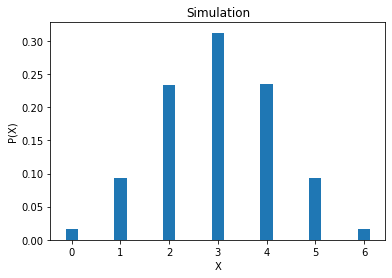
\includegraphics[width=0.58\textwidth]{assignment1.png}
\end{center}
\end{figure}
\begin{figure}
\begin{center}
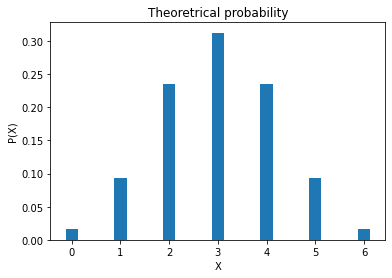
\includegraphics[width=0.58\textwidth]{assignment-1.png}
\end{center}
\end{figure}

\end{document}